\documentclass{JNUexp}
\courseName{Linux 环境程序设计}
\expName{实验 5 常用开发工具}
\expDate{2017.11.14}
\className{计科1404}
\studentName{阎覃}
\studentId{1030414414}

\graphicspath{ {images/} }

\usepackage[hidelinks]{hyperref}
\begin{document} 

\section{实验目的}
\begin{itemize}
    \item 掌握 C 语言编译的基本用法;
    \item 掌握 gdb 调试工具的基本用法;
    \item 理解 make 工具的功能,学会编制 makefile 的方法。
    
\end{itemize}

\section{实验内容}
\begin{itemize}
    \item 利用 gcc 命令编译 C 语言程序,使用不同选项,观察并分析显示结果
    \item 用 gdb 命令调试一个编译后的 C 语言程序
    \item 编写一个由多个文件构成的 C 语言程序,编制 makefile,运行 make 工具进行维护
\end{itemize}
\section{实验步骤及运行情况}
%%%%%%%%%%%%%%%%%%%%%%%%%%%%%%%%%%%%%%%%%%%%%%%%%%%%%%%%%
%   1
%%%%%%%%%%%%%%%%%%%%%%%%%%%%%%%%%%%%%%%%%%%%%%%%%%%%%%%%%
\begin{problem}
    改写例 6.1,使用下列选项对它进行编译:-I,-D,-E,-c,-o,-l
\end{problem}

\begin{answer}
    下面分别是tmp/testI.h和hello.c的源代码:

    \lstinputlisting[language=C,title=tmp/testI.h]{../src/tmp/testI.h}    
    \lstinputlisting[language=C,title=hello.c]{../src/hello.c}    

    \subparagraph{-I} 指定头文件的目录
    \begin{lstlisting}[language=sh]
gcc -I ./tmp hello.c
    \end{lstlisting}
    指定./tmp目录后找不到头文件的报错就消失了。

    \subparagraph{-D} 定义一个宏,若不指定值则为1 
    \begin{lstlisting}[language=sh]
gcc -I ./tmp -D DOPTION='"testing -D"' -D fatal hello.c
    \end{lstlisting}
    这里存在两次重复定义的警告,第一次将\lstinline{1}重定义为\lstinline{abc},第二次为\lstinline{please call Lawrence for help}


    \subparagraph{-E} 只对文件进行预处理,不进行编译、链接,生成的结果送标准输出,即只运行预编译器 \\
    \begin{lstlisting}[language=sh]
gcc -I ./tmp -D DOPTION='"testing -D"' -E hello.c
    \end{lstlisting}
    可以发现原来没定义的DOPTION等宏都被替换了。
    \begin{figure}[h]
        \centering
        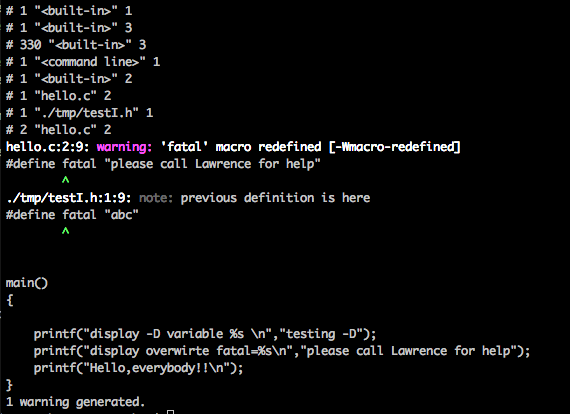
\includegraphics[width=0.7\textwidth]{1}
        \caption{预编译后的结果}
    \end{figure}

    \subparagraph{-c} 只把源文件编译成目标代码.o
    \begin{lstlisting}[language=sh]
gcc -I ./tmp -D DOPTION='"testing -D"' -c hello.c
    \end{lstlisting}
    \begin{figure}[h]
        \centering
        
\includegraphics[width=0.7\textwidth]{2}
        \caption{编译成目标文件}
    \end{figure}

    \subparagraph{-o file1} 编译成可执行文件file1。
    \begin{lstlisting}[language=sh]
gcc -I ./tmp -D DOPTION='"testing -D"' -o abc hello.c
    \end{lstlisting}
    \begin{figure}[h]
        \centering
        
\includegraphics[width=0.7\textwidth]{3}
        \caption{编译成可执行文件}
    \end{figure}

    \subparagraph{-llib} 指定程序要链接的库为lib
    \begin{lstlisting}[language=sh]
gcc -I ./tmp -D DOPTION='"testing -D"' -llib hello.c
    \end{lstlisting}

\end{answer}

%%%%%%%%%%%%%%%%%%%%%%%%%%%%%%%%%%%%%%%%%%%%%%%%%%%%%%%%%
%   2
%%%%%%%%%%%%%%%%%%%%%%%%%%%%%%%%%%%%%%%%%%%%%%%%%%%%%%%%%
\begin{problem}
    完成对思考题 6.5 的调试
\end{problem}

\begin{answer}
    由于macOS 没有预装gdb,所以要通过HomeBrew进行安装。
    \begin{lstlisting}[language=sh]
brew install gdb
    \end{lstlisting}

    程序如图所示
    \lstinputlisting[language=c,title=badprog.c]{../src/badprog.c}
    
    程序有一个参数,-b 访问越界内存,-f 访问清空后的内存。\\
\end{answer}

\begin{image}
    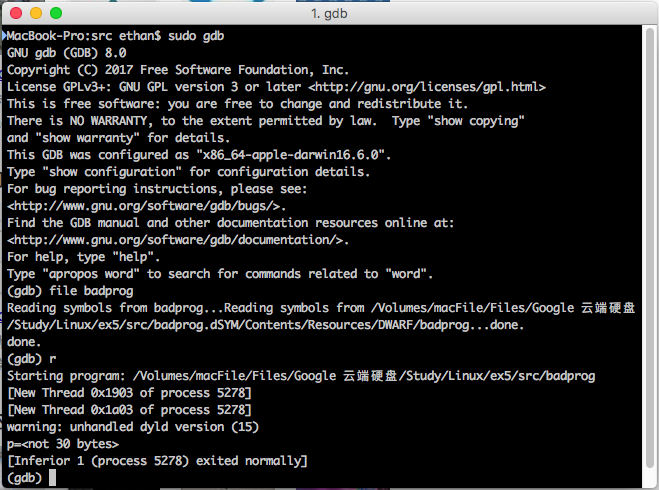
\includegraphics[width=0.7\textwidth]{4}
\end{image}

%%%%%%%%%%%%%%%%%%%%%%%%%%%%%%%%%%%%%%%%%%%%%%%%%%%%%%%%%
%   3
%%%%%%%%%%%%%%%%%%%%%%%%%%%%%%%%%%%%%%%%%%%%%%%%%%%%%%%%%
\begin{problem}
    完成对思考题 6.6 的调试
\end{problem}

\begin{answer}
    程序如图所示
    \lstinputlisting[language=c,title=callstk.c]{../src/callstk.c}
\end{answer}

\begin{image}
    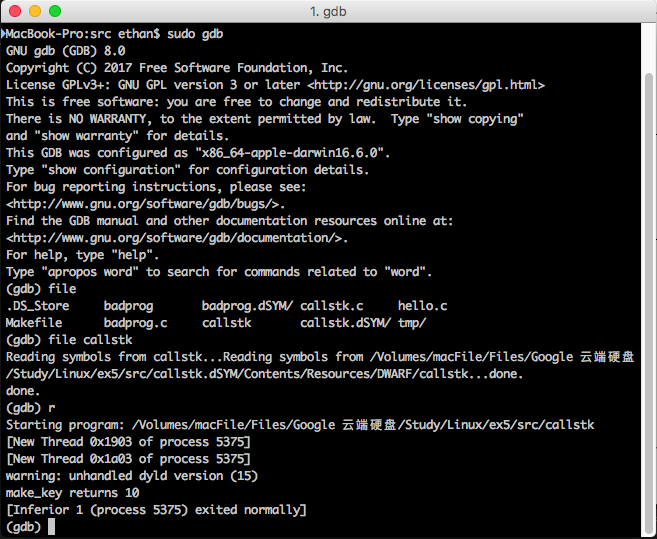
\includegraphics[width=0.7\textwidth]{5}
\end{image}

%%%%%%%%%%%%%%%%%%%%%%%%%%%%%%%%%%%%%%%%%%%%%%%%%%%%%%%%%
%   4
%%%%%%%%%%%%%%%%%%%%%%%%%%%%%%%%%%%%%%%%%%%%%%%%%%%%%%%%%
\begin{problem}
    完成对思考题 6.9 的编制,并使用 make 命令进行维护
\end{problem}

\begin{answer}
    Makefile如图所示
    \lstinputlisting[language={[gnu]make},title=Makefile]{../src/Makefile}
\end{answer}

\newpage
\section{实验体会}
虽然很早就会用gcc编译c程序,但是从没有过如此详细的了解gcc的各种参数。过去都是通过IDE来开发程序,
通过这次学习我了解到gcc编译器其实支持许多功能,也认识到IDE工作的原理,以往在IDE中设定的头文件等
工作目录是怎么加载的。通过gdb 可以调试程序,gdb的功能十分强大,这次试验也仅仅是一次体验。make是
一个很常用的工具,通过编写Makefile ,我们只需要make就可以编译整个工程。

\vfill

实验报告采用 \LaTeX 编写,代码托管至GitHub:\\
\url{https://github.com/Ethan-yt/JNU-Linux-exp}

\end{document}